
%%%%%%%%%%%%%%%%%%%%%%%%%%%%%%%%%%%%%%%%%%%%%%%%%%%%%%%%%%%%%%%%%%%%%%%%%%%%%%%%
%%%%%%%%%%%%%%%%%%%%%%%%%%%%%%%%%%%%%%%%%%%%%%%%%%%%%%%%%%%%%%%%%%%%%%%%%%%%%%%%

%%%%%%%%%%%%%%%%%%%%%%%%%%%%%%%%%%%%%%%%%%%%%%%%%%%%%%%%%%%%%%%%%%%%%%%%%%%%%%%%
%%%%%%%%%%%%%%%%%%%%%%%%%%%%%%%%%%%%%%%%%%%%%%%%%%%%%%%%%%%%%%%%%%%%%%%%%%%%%%%%
\clearpage
\section{Usando o breque da música}
\label{sec:UsandoBreak}
\index{Musicalidade!Breque}

Na Seção \ref{sec:percepcionbreak} foram mostradas algumas dicas 
úteis para poder antecipar os breques na música.
Com essa informação um dançarino pode incorporar este aspecto da música na sua dança.

Nesta seção apresentaremos um conjunto de sugestões  
sobre como interpretar os breques\footnote{Estas 
sugestões entram na categoria de ``mapeamento'' de aspectos da música, 
explicado na Figura \ref{fig:interpretacion-corporal} da Pag. \pageref{fig:interpretacion-corporal}.}.
Dentro da lista de recomendações de mapeamento entre os aspectos de nosso movimento e as pausas da música, 
temos que:
\begin{itemize}
\item Quando acontece uma pausa (breque) total na música 
é interessante acompanhar este evento realizando também uma pausa total em nossos movimentos.
\item Se o breque acontece e um solo melódico ou percussivo preenche a pausa,
então nós temos duas opções: 
\begin{itemize}
\item desprezar o solo e permanecer inativos\footnote{Se suspeitamos que o solo é curto, é mais fácil esperar que inventar.} ou
\item utilizar o solo musical e realizar um solo de dança\footnote{Se o solo musical promete ser longo, podemos arriscar fazer alguma graça.};
ou seja realizar uma dança que incorpore aspectos do solo musical,
de modo que fique evidente que é um intermédio entre duas propostas de movimentos,
a anterior e a posterior ao breque.
\end{itemize}
\item Se decidimos dançar o solo no breque, 
então lembremos que é comum 
\begin{itemize}
\item mapear os movimentos de pés ou de deslocamento com as mudanças do ritmo 
(do acompanhamento ou da melodia) e 
\item mapear movimentos corporais quase sem deslocamento a aspectos da melodia (mudança de tons, tensão, articulação, etc.).
\end{itemize}
Além disso, se o solo no breque é o suficientemente longo, 
existe a possibilidade de misturar ambas técnicas usando movimentos corporais e alguns deslocamentos.
\item Também poderíamos simplesmente dançar no silencio da pausa, colocando um movimento corporal sem deslocamento 
para não perder a inercia de nossos movimento até iniciar a seguinte frase musical.
\item Quando temos um par de dança e decidimos usar a pausa na música,
nós podemos dançar separados ou usando um abraço.
\begin{itemize}
\item Se o abraço é \hyperref[def:closed-position]{\textbf{fechado}}, os movimentos do condutor estarão mais limitados 
e este deverá conduzir os movimentos do seguidor.
\item Se o par de dança está separado ou o abraço é \hyperref[def:closed-position]{\textbf{aberto}}, 
o seguidor e o condutor tem mais liberdade de movimento, 
de modo que se eles desejam podem executar cada um seus movimentos de forma independentemente.
\end{itemize}
Entre os movimentos que poderíamos usar no breque, estão por exemplo: 
um samba no pé, um bamboleio circular de quadril (no plano axial), um balanço de ombros (no plano frontal), etc. 
\item Uma vez finalizado o solo, é mais fácil iniciar a seguinte frase musical
no primeiro \hyperref[subsec:perceberTF1]{\textbf{tempo forte}}. 
Ao finalizar o solo devemos ter bem definido o peso do corpo num pé 
para poder ter rapidez em iniciar a seguinte frase.
\item É interessante esperar com os pés próximos o inicio da frase posterior a um breque; 
pois quando estão separados será mais difícil iniciar a frase musical com um passo com expressividade,
dado que nosso passo tem um limite o qual diminui com a distancia inicial entre nossos pés.
\end{itemize}

No Exemplo \ref{ex:breakvarios} indicamos um conjunto de músicas 
que são ótimas para o treinamento das pausas de forma unipessoal,
pois tem uma grande quantidade de breques e solos.
\begin{example}[Músicas com muitos breques]
\label{ex:breakvarios}
Em todos os exemplos listados, os breques acontecem na linha melódica principal e no acompanhamento,
enquanto que o cantor faz solos ``falados''.
\begin{itemize}
\item ``Idade não é documento'' interpretado por Moreira da silva.
\item ``Jogando com o capeta'' interpretado por Moreira da silva.
\item ``Na subida do morro'' interpretado por Moreira da silva. 
O primeiro breque é feminino.
\end{itemize}
Dado que a voz falada tem um tom quase uniforme e não poderia ser considerada preponderantemente melódica,
se sugere, sim se deseja dançar o solo, que se aproveite só a parte rítmica da voz.
\end{example}

Outras músicas com breques podem ser encontradas nos Exemplos \ref{ex:breakmasculinos},
\ref{ex:breakfeminino} e 
\ref{ex:breaksincopados}.

\begin{figure}[h]
\index{Tira cómica}
    \centering
    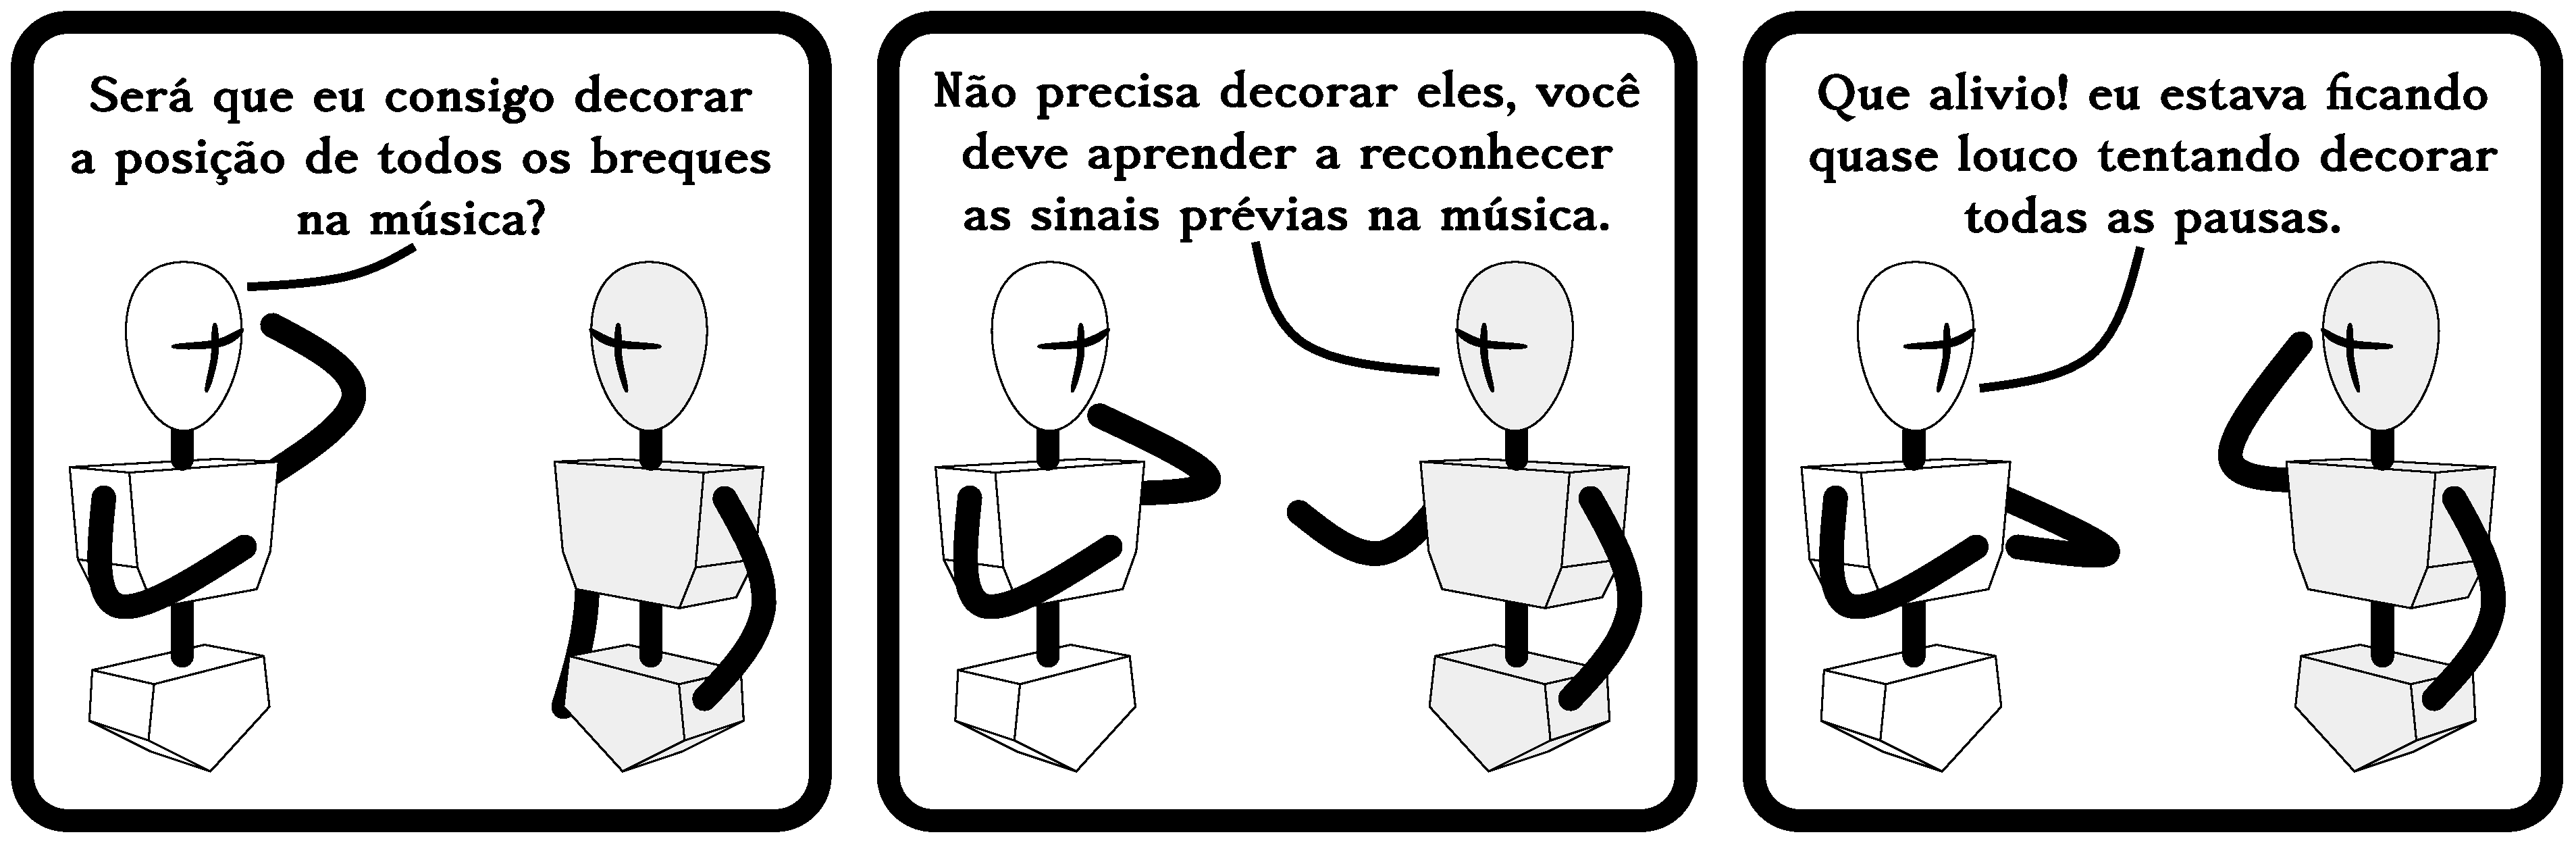
\includegraphics[width=\textwidth]{comic/tira-breque2.eps}
    %\caption{Contando tempos coregráficos.}
    %\label{fig:contagemtempocoreografico}
\end{figure}

